\documentclass[11pt,preprint, authoryear]{elsarticle}

\usepackage{lmodern}
%%%% My spacing
\usepackage{setspace}
\setstretch{1.2}
\DeclareMathSizes{12}{14}{10}{10}

% Wrap around which gives all figures included the [H] command, or places it "here". This can be tedious to code in Rmarkdown.
\usepackage{float}
\let\origfigure\figure
\let\endorigfigure\endfigure
\renewenvironment{figure}[1][2] {
    \expandafter\origfigure\expandafter[H]
} {
    \endorigfigure
}

\let\origtable\table
\let\endorigtable\endtable
\renewenvironment{table}[1][2] {
    \expandafter\origtable\expandafter[H]
} {
    \endorigtable
}


\usepackage{ifxetex,ifluatex}
\usepackage{fixltx2e} % provides \textsubscript
\ifnum 0\ifxetex 1\fi\ifluatex 1\fi=0 % if pdftex
  \usepackage[T1]{fontenc}
  \usepackage[utf8]{inputenc}
\else % if luatex or xelatex
  \ifxetex
    \usepackage{mathspec}
    \usepackage{xltxtra,xunicode}
  \else
    \usepackage{fontspec}
  \fi
  \defaultfontfeatures{Mapping=tex-text,Scale=MatchLowercase}
  \newcommand{\euro}{€}
\fi

\usepackage{amssymb, amsmath, amsthm, amsfonts}

\def\bibsection{\section*{References}} %%% Make "References" appear before bibliography


\usepackage[round]{natbib}

\usepackage{longtable}
\usepackage[margin=2.3cm,bottom=2cm,top=2.5cm, includefoot]{geometry}
\usepackage{fancyhdr}
\usepackage[bottom, hang, flushmargin]{footmisc}
\usepackage{graphicx}
\numberwithin{equation}{section}
\numberwithin{figure}{section}
\numberwithin{table}{section}
\setlength{\parindent}{0cm}
\setlength{\parskip}{1.3ex plus 0.5ex minus 0.3ex}
\usepackage{textcomp}
\renewcommand{\headrulewidth}{0.2pt}
\renewcommand{\footrulewidth}{0.3pt}

\usepackage{array}
\newcolumntype{x}[1]{>{\centering\arraybackslash\hspace{0pt}}p{#1}}

%%%%  Remove the "preprint submitted to" part. Don't worry about this either, it just looks better without it:
\makeatletter
\def\ps@pprintTitle{%
  \let\@oddhead\@empty
  \let\@evenhead\@empty
  \let\@oddfoot\@empty
  \let\@evenfoot\@oddfoot
}
\makeatother

 \def\tightlist{} % This allows for subbullets!

\usepackage{hyperref}
\hypersetup{breaklinks=true,
            bookmarks=true,
            colorlinks=true,
            citecolor=blue,
            urlcolor=blue,
            linkcolor=blue,
            pdfborder={0 0 0}}


% The following packages allow huxtable to work:
\usepackage{siunitx}
\usepackage{multirow}
\usepackage{hhline}
\usepackage{calc}
\usepackage{tabularx}
\usepackage{booktabs}
\usepackage{caption}


\newenvironment{columns}[1][]{}{}

\newenvironment{column}[1]{\begin{minipage}{#1}\ignorespaces}{%
\end{minipage}
\ifhmode\unskip\fi
\aftergroup\useignorespacesandallpars}

\def\useignorespacesandallpars#1\ignorespaces\fi{%
#1\fi\ignorespacesandallpars}

\makeatletter
\def\ignorespacesandallpars{%
  \@ifnextchar\par
    {\expandafter\ignorespacesandallpars\@gobble}%
    {}%
}
\makeatother

\newlength{\cslhangindent}
\setlength{\cslhangindent}{1.5em}
\newenvironment{CSLReferences}%
  {\setlength{\parindent}{0pt}%
  \everypar{\setlength{\hangindent}{\cslhangindent}}\ignorespaces}%
  {\par}


\urlstyle{same}  % don't use monospace font for urls
\setlength{\parindent}{0pt}
\setlength{\parskip}{6pt plus 2pt minus 1pt}
\setlength{\emergencystretch}{3em}  % prevent overfull lines
\setcounter{secnumdepth}{5}

%%% Use protect on footnotes to avoid problems with footnotes in titles
\let\rmarkdownfootnote\footnote%
\def\footnote{\protect\rmarkdownfootnote}
\IfFileExists{upquote.sty}{\usepackage{upquote}}{}

%%% Include extra packages specified by user

%%% Hard setting column skips for reports - this ensures greater consistency and control over the length settings in the document.
%% page layout
%% paragraphs
\setlength{\baselineskip}{12pt plus 0pt minus 0pt}
\setlength{\parskip}{12pt plus 0pt minus 0pt}
\setlength{\parindent}{0pt plus 0pt minus 0pt}
%% floats
\setlength{\floatsep}{12pt plus 0 pt minus 0pt}
\setlength{\textfloatsep}{20pt plus 0pt minus 0pt}
\setlength{\intextsep}{14pt plus 0pt minus 0pt}
\setlength{\dbltextfloatsep}{20pt plus 0pt minus 0pt}
\setlength{\dblfloatsep}{14pt plus 0pt minus 0pt}
%% maths
\setlength{\abovedisplayskip}{12pt plus 0pt minus 0pt}
\setlength{\belowdisplayskip}{12pt plus 0pt minus 0pt}
%% lists
\setlength{\topsep}{10pt plus 0pt minus 0pt}
\setlength{\partopsep}{3pt plus 0pt minus 0pt}
\setlength{\itemsep}{5pt plus 0pt minus 0pt}
\setlength{\labelsep}{8mm plus 0mm minus 0mm}
\setlength{\parsep}{\the\parskip}
\setlength{\listparindent}{\the\parindent}
%% verbatim
\setlength{\fboxsep}{5pt plus 0pt minus 0pt}



\begin{document}



\begin{frontmatter}  %

\title{Night Lights and Noisy Data - Using Machine Learning to Better
Detect Human-Generated Lights}

% Set to FALSE if wanting to remove title (for submission)




\author[Add1]{Johannes Coetsee}
\ead{19491050@sun.ac.za - https://github.com/Coetsee}





\address[Add1]{Stellenbosch University}


\begin{abstract}
\small{
In recent years, researchers in the social sciences have increasingly
relied on the usage of alternative sources of data with which to answer
research questions. One of these alternative avenues - remote sensing
and satellite data - offers unique potential for socioeconomic research.
A prominent and widely popular example is the Stable Lights product,
derived from the Defense Meteorological Satellite Program's (DMSPs)
Operational Linescan System (OLS), which captures nighttime luminosity
of lights data worldwide. Despite its usefulness, this source of data
suffers from some potentially severe accuracy-related challenges,
however, including the presence of background noise especially in areas
that display lower nightlight luminosity (NL). The following paper
emphasises the latter challenge, and implements an adjusted version of
the noise-filtering methodology proposed by Määttä \& Lessmann
(\protect\hyperlink{ref-maatta}{2019}), in which the authors use a
variety of derived and externally-sourced remote sensing inputs to
inform a Random Forest (RF) algorithm that categorises night-light data
as being human-generated or not. This methodology proves fruitful in
separating useful data from noise, thereby addressing some of the
challenges related to the Stable Lights product.
}
\end{abstract}

\vspace{1cm}

\begin{keyword}
\footnotesize{
Remote Sensing \sep Night Lights \sep Random Forest
\sep DMSP-OLS \\ \vspace{0.3cm}
}
\end{keyword}
\vspace{0.5cm}
\end{frontmatter}



%________________________
% Header and Footers
%%%%%%%%%%%%%%%%%%%%%%%%%%%%%%%%%
\pagestyle{fancy}
\chead{}
\rhead{Advanced Cross Section Econometrics - January 2022}
\lfoot{}
\rfoot{\footnotesize Page \thepage}
\lhead{}
%\rfoot{\footnotesize Page \thepage } % "e.g. Page 2"
\cfoot{}

%\setlength\headheight{30pt}
%%%%%%%%%%%%%%%%%%%%%%%%%%%%%%%%%
%________________________

\headsep 35pt % So that header does not go over title




\hypertarget{introduction}{%
\section{\texorpdfstring{Introduction
\label{Introduction}}{Introduction }}\label{introduction}}

In recent years, the usage of remote sensing data has expanded
exponentially due to its potential for new and diverse applications in
socioeconomic research. These data sources are often deemed largely
objective and free from standard sample selection challenges, and is
thereby suitable as a proxy in a broad array of studies that require the
usage of potentially unreliable or unavailable data. This advantage is
especially pertinent in parts of the developing world, where reliable
data can be relatively hard to come by. One of the most prominent remote
sensing data avenues has been the satellite-derived nightlight
luminosity data sets, with luminosity often being used as a proxy for
important measures such as population counts\footnote{See, for instance,
  Mellander, Lobo, Stolarick \& Matheson
  (\protect\hyperlink{ref-mellander2015night}{2015}).}, economic
activity and growth \footnote{Elvidge, Baugh, Kihn, Kroehl, Davis \&
  Davis (\protect\hyperlink{ref-elvidge1997}{1997a}); Henderson,
  Storeygard \& Weil (\protect\hyperlink{ref-henderson2012}{2012}) and
  Chen \& Nordhaus (\protect\hyperlink{ref-chen2011}{2011}) are
  prominent examples.} and regional inequality indices.\footnote{Such as
  in Ivan, Holobâcă, Benedek \& Török
  (\protect\hyperlink{ref-ivan2020nlinequality}{2020}) and Mveyange
  (\protect\hyperlink{ref-mveyange2015}{2015}).} One of the most common
nightlight luminosity data sets, the `Stable Lights' product derived
from the Defense Meteorological Satellite Program's (DMSPs) Operational
Linescan System (OLS), has seen a vast array of applications. However,
there remains questions surrounding its reliability and accuracy. This
paper emphasises some of these shortcomings. Most prominently, DMSP-OLS
has difficulty in separating background noise from night lights
generated from human-generated light, especially in areas that display
lower levels of night light intensity. This presents an obvious and
difficult-to-overcome challenge: analyses that attempt to use Stable
Lights as a proxy for economic activity, for instance, may either
exaggerate or understate economic activity in these low-luminous areas,
which proves difficult to rectify.

In addition to pointing out these and other shortcomings, this paper
also attempts to address the challenge of background noise by applying a
filtering technique to identify and separate nightlights emitted by
humans from those emitted by other sources. This filtering process is
based on the methodology for deriving the `Local Human Lights' product
by Määttä \& Lessmann (\protect\hyperlink{ref-maatta}{2019}), and relies
on a Random Forest (RF) machine learning algorithm for classification.
Whilst drawing largely on Määttä \& Lessmann
(\protect\hyperlink{ref-maatta}{2019}), there remains distinct
differences in approach between our methodology and theirs. Most
prominently, Määttä \& Lessmann (\protect\hyperlink{ref-maatta}{2019})
apply their filter on the entire world, whilst including some inputs
that are region-specific. In contrast, we apply their methodology only
to the South African subset of data, which carry some implications in
terms of application. This, and other deviations, will be explicated on
in more detail in section \ref{Methodology}, however. The rest of the
paper is laid out as follows: section \ref{problem} briefly discusses
some of the primary challenges with the DMSP-OLS data, whilst section
\ref{Methodology} discusses the noise-filtering methodology and the data
inputs needed for the RF algorithm. Section \ref{Results} presents some
results and visualizations, and section \ref{Discussion} concludes.

\begin{figure}[H]
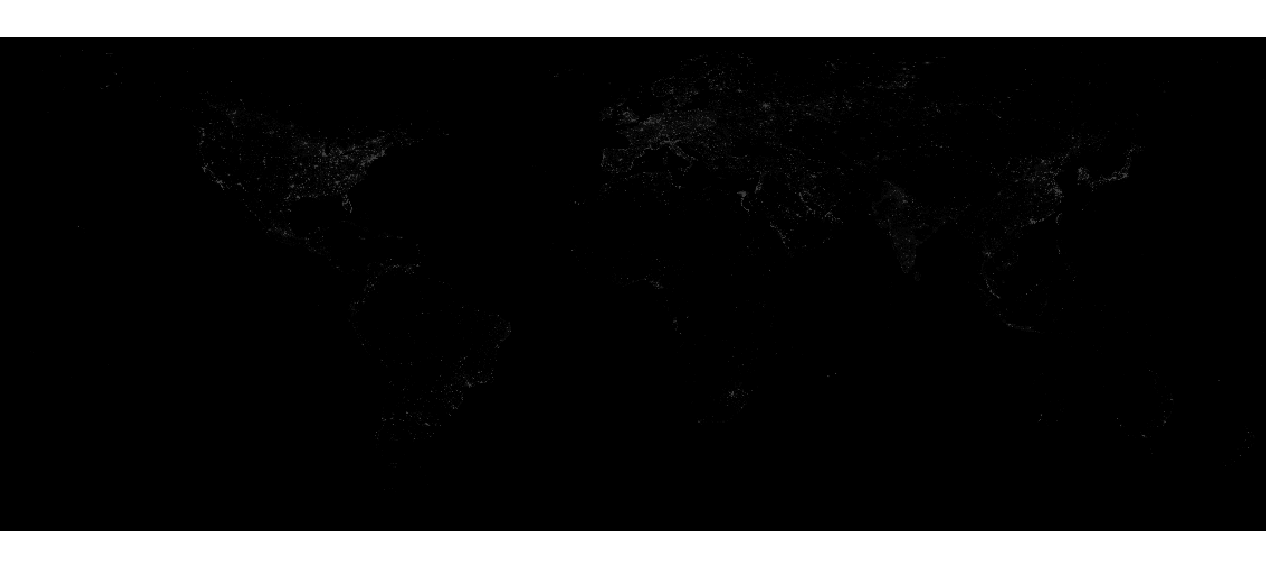
\includegraphics[width=1\linewidth]{figures/stable_full} \caption{\label{stable} The Raw Stable Lights Image}\label{fig:stable}
\end{figure}

\hypertarget{night-light-data-and-noise}{%
\section{\texorpdfstring{Night Light Data and Noise
\label{problem}}{Night Light Data and Noise }}\label{night-light-data-and-noise}}

The Stable Lights product is one of the most popular remote sensing data
sets in circulation. This is due largely to its numerous uses described
in the previous section, but also because of its public availability and
ease of use. The primary product is derived from the DMSP-OLS nighttime
light emissions data, which is captured by satellites that measure
global light emissions at night. The raw satellite data is processed by
the National Oceanic and Atmospheric Administration (NOAA) in
collaboration with the American National Geophysical Data Center (NGDC),
and involves the manipulation of the raw data to compensate for cloud
coverage, ephemeral events and some other sources of background noise.
The compiled Stable Lights product is thus a yearly composite of datum
consisting out of a grid of numbers ranging from 0 (no emission) to 63
(the maximum emission readable by satellite sensors), where each cell,
or pixel, reflects the light emissions of an area approximately 0.86
square kilometers in size at the equator. The DMSP-OLS series consists
of 6 satellites collectively active over the period 1992-2013, with some
satellites capturing data across the same years.

Despite its usefulness, and despite attempts to minimize the potential
for noise, the stable lights product has some notable limitations.
First, its radiometric resolution (6-bit data with values ranging only
from 0 to 63) is relatively low and therefore not sensitive to changes
in emissions, whilst it also has a fairly large spatial resolution.
These two factors limit the accuracy in emissions-measurement. A further
and prominent limitation is concerned with the intensity and extent of
lit-up areas, where pixel saturation and the blooming effect complicate
the direct delimiting of especially urban regions. Saturation here
refers to the upper-bound luminosity value of 63, meaning that certain
highly-lit areas will show no variation of emissions over time. The
blooming effect is a well-known phenomenon wherein the identification of
a lit area is consistently larger than its corresponding
settlement.\footnote{This occurs due to the coarse spatial resolution of
  the OLS sensors, large overlap in the footprints of adjacent OLS
  pixels, and the accumulation of geolocation errors in the compositing
  process.} Similarly, the sensors that capture these emissions differ
across satellites, and can also suffer from sensory degradation, thereby
not necessarily being directly comparable. In order to accurately
compare NL emissions across years, one would have to perform
intercalibration, something that the DMSP-OLS data sets do not contain
on-board (Elvidge, Baugh, Kihn, Kroehl, Davis \& Davis
(\protect\hyperlink{ref-elvidge1997relation}{1997b}); Elvidge, Baugh,
Zhizhin \& Hsu (\protect\hyperlink{ref-elvidge2013viirs}{2013})).

The most prominent difficulty, however, relates to the amount of noise
in the lower end of the light distribution, due in part to the blooming
effect mentioned above. A common solution to the problem of noise is to
either filter out data below a certain threshold, or set those values to
an arbitrarily small number between 0 and 1. This is, however, a
quick-and-easy solution that effectively throws away potentially
important and insightful information. Figure \ref{stable_no_noise} below
displays the difference between the raw Stable Lights image, which
includes suspected noise at the lower end of the light spectrum, and the
image where all cell values below 6 are transformed to 0.1, an arbitrary
number often used in these analyses. Even when comparing the images
visually, it is evident that large swaths of data on the peripheries of
urban centers are discarded. In addition to the arbitrarily-chosen
threshold and replacement values, the loss of variability in cell values
makes it especially difficult to perform statistical analyses in a large
variety of cases.

\begin{figure}[H]
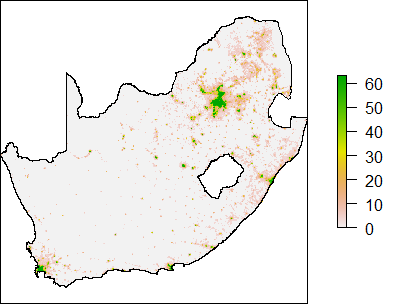
\includegraphics[width=0.5\linewidth]{figures/stable_SA} 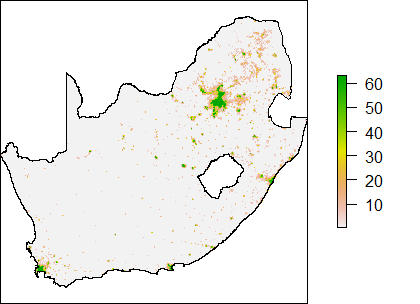
\includegraphics[width=0.5\linewidth]{figures/stable_SA_noise_filtered} \caption{\label{stable_no_noise} Left - Raw Stable Lights; Right - Noise Discarded}\label{fig:stable_no_noise}
\end{figure}

The latter challenge constitutes the primary emphasis of the methodology
implemented in the subsequent sections. However, the paragraph above
should serve as a reminder that there exists other accuracy-related
problems with the DMSP-OLS data sets.

\hypertarget{method-and-data}{%
\section{\texorpdfstring{Method and Data
\label{Methodology}}{Method and Data }}\label{method-and-data}}

We follow the methodology advanced by Määttä \& Lessmann
(\protect\hyperlink{ref-maatta}{2019}), where the authors propose a
process of noise filtering with the aim to more accurately identify
\emph{human-emitted} nightlights. Successful implementation would negate
the need to drop observations believed to be noise. If one can
accurately discern between which lights are human generated and which
ones are not, one can remove only those classified as noise and thereby
prevent data loss. The process the authors propose utilises a Random
Forest (RF) machine learning algorithm to predict where places have a
higher likelihood of displaying human-generated light activity, based on
satellite data of built-up and settlement areas. Määttä \& Lessmann
(\protect\hyperlink{ref-maatta}{2019}) develop two distinct products -
Global Human Lights and Local Human Lights - for the F15 satellite in
2001. While the global product minimizes bias arising from the usage of
regional information, the local product maximizes predictive accuracy.
The local and global products differ largely due to the incorporation of
a a battery of local light variables derived from the average visible
lights and the percentage frequency of light detection products for the
local product. This greatly improves the detection of lights generated
by humans, especially on the African continent. As our emphasis is on
more accurate prediction, and also only on the South African NL subset,
we are most interested in replicated and extending the methodology for
the local product. Before delving into more detail regarding the
employed algorithm, however, it would be useful to first briefly discuss
the primary data inputs.

\hypertarget{data}{%
\subsection*{Data}\label{data}}
\addcontentsline{toc}{subsection}{Data}

Table \ref{variable_table} below gives an overview of the most important
variables used as inputs. The Global Human Settlement Layer (GHSL)
\emph{built-up} grid - satellite-derived images of the world based on
Landsat satellites - is used to classify whether a certain area is more
likely to contain human generated light, as humans are active in areas
where there are buildings and infrastructure. The built-up data is thus
the measure whereby the algorithm classifies whether lit pixels can be
classified as human generated or not.\footnote{For more on the GHSL
  methodology, consult Pesaresi, Ehrlich, Ferri, Florczyk, Freire,
  Halkia, Julea, Kemper, Soille, Syrris \& others
  (\protect\hyperlink{ref-pesaresi2016operating}{2016}).} The second and
third variables constitute the two primary DMSP-OLS products released by
NOAA, and is also the most crucial inputs in the filtering
methodology.\footnote{These two products, together with Stable Lights,
  constitute all of the publicly available DMSP-OLS data.} This is due
to the fact that the subsequent variables are derived from them. The
\emph{local noise} variable is used to identify those areas where
background noise is systematically larger than some threshold, and
consists out of the number of pixels in a window of 499 by 499 pixels
below this threshold.\footnote{We follow Määttä \& Lessmann
  (\protect\hyperlink{ref-maatta}{2019}) in choosing the upper bound
  threshold value of 6 so as to be most strict in what is considered
  noise.} The \emph{local detections} counts the number of pixels where
zero light is detected in a 399 by 399 window around a pixel. The rest
of the variables are generated to be regional input variables that more
closely describe the characteristics of luminosity surrounding a
specific pixel. By varying the size of the area around a pixel, one more
accurately accounts for spatial correlations in light that is human
generated.

\begin{table}
\begin{center}
\begin{tabular}{ |l|l|l| }
 \hline
 Input & Source & Description  \\
 \hline
  built up & GHSL & Landsat satellite images of built-up areas \\
  avg light & DMSP-OLS & average light per pixel over a year \\
  freq light & DMSP-OLS & proportion of days where light is detected per pixel \\
  local noise & Derived from DMSP-OLS & number of pixels below threshold in avg light image \\
  local detections & Derived from DMSP-OLS & accounts for regional differences in freq light \\
  lm freq 5 & Derived from DMSP-OLS & average of freq light in a 5 by 5 pixel area \\
  lm avg 25 & Derived from DMSP-OLS & average of avg light in a 25 by 25 pixel area \\
  lm freq 99 & Derived from DMSP-OLS & average of freq light in a 99 by 99 pixel area \\
  lm avg 199 & Derived from DMSP-OLS & average of avg light in a 199 by 199 pixel area \\
  \hline
\end{tabular}
\caption{Data Inputs}
\label{variable_table}
\end{center}
\end{table}

The derived variables in Table \ref{variable_table} are displayed in
Figure \ref{local_images} below. These are the local input images for
the F18 satellite, which recorded light emissions in 2011. For each
iteration of the algorithm across the three satellites, these 6
variables are derived anew.

\begin{figure}[H]
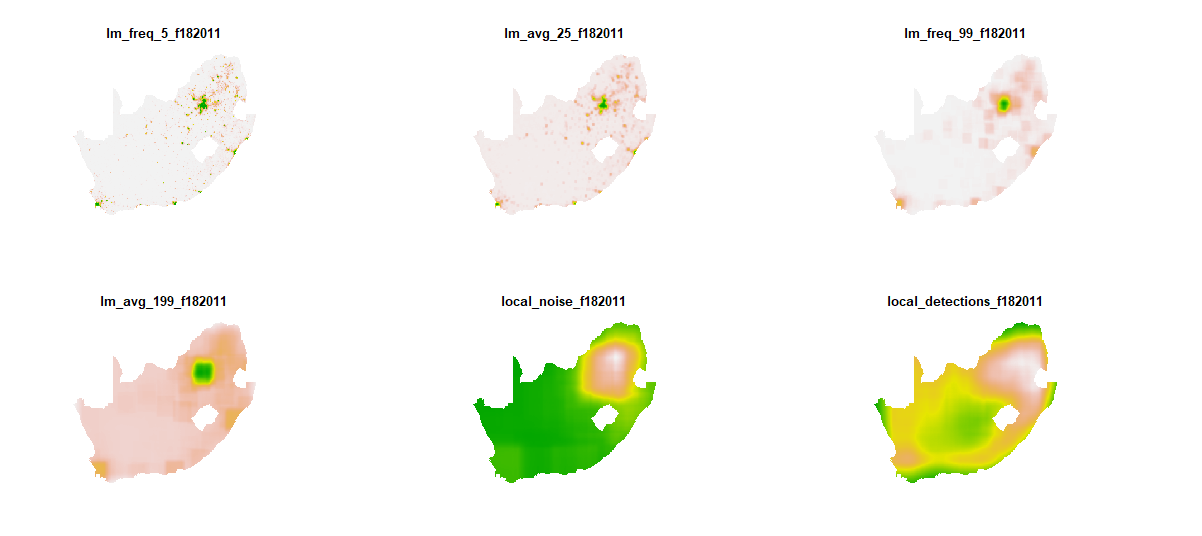
\includegraphics[width=1\linewidth]{figures/local_inputs} \caption{\label{local_images} Local Image Inputs}\label{fig:local_images}
\end{figure}

\hypertarget{methodology}{%
\subsection*{Methodology}\label{methodology}}
\addcontentsline{toc}{subsection}{Methodology}

Määttä \& Lessmann (\protect\hyperlink{ref-maatta}{2019})'s methodology
necessitates four primary steps: First, the regional night light
variables are created from the original \emph{avg light} and \emph{freq
light} DMSP-OLS products. Second, the world map is divided in various
sub-regions, as the random forest algorithm will be run on each
sub-region separately. All the variable images are cropped into
2000-pixel square sub-regions, which equates to about 3.4 million
\(km^2\). Each sub-region further consists of approximately 4 million
rows of datum, whilst the model is trained on a 10\% subsample. However,
running the algorithm on separate sub-regions introduces variability in
the classification rule, which, in turn, translates to discontinuous
jumps in predicted probabilities at the borders of each region. To
address this, each window is jittered in small steps of 250 pixels, and
the algorithm is applied for each of the jittered steps. The results are
then averaged to smooth away border effects. In step three, probability
thresholds are derived for each region, and subsequently used to create
image masks that indicate whether a pixel is above the probability
threshold of it being human generated or not. The final step entails
overlaying the original \emph{avg light} image with the masks for each
region, and then creating a mosaic from all of the sub-regions to create
the final local product.

The random forest algorithm is used to predict the probability of lights
being of human origin or not. It does this by using the built up data as
a proxy for human activity. One cannot merely use the built up data
directly to filter out noise, as human-generated light can also be
generated in areas that are not built up, and conversely, some built-up
areas do not emit any lights (like country roads, for instance). This
means therefore that measures commonly used to assess the prediction
accuracy of a random forest - such as the accuracy and F1 scores -
cannot be used as is, as these scores would merely relate how accurately
lights relate to built-up area. Määttä \& Lessmann
(\protect\hyperlink{ref-maatta}{2019}) instead propose introducing a
tolerance threshold, where pixels are classified in order of highest
probability, until the threshold level of the \emph{avg light} pixels is
reached. This inevitably implies that a choice must be made about the
threshold value; if the threshold is higher, less pixels will be
classified as lit up, and \emph{vice versa}. In fact, there are numerous
choices that trade off necessity with more accurate human light
detection. The choice of threshold being one of them, but so also the
size of the steps that smooths the border effects; the size of the
sub-region windows; which regional light variables to include; at which
probability level to classify lights as definitely human-generated (the
classification rule); as well as a backstopping rule.\footnote{These
  choices are in addition to the standard parameter-decisions required
  for a random forest. In our case, the most prominent parameters are
  chosen as follows: mtry = 1 (due to computational limitations),
  splitrule = ``gini'', min.node.size = 10, num\_trees = 200, and trees
  are always split on the \emph{avg} and \emph{pct} variables.} It is
therefore important to note where our methodological decisions diverge
from the default values proposed by Määttä \& Lessmann
(\protect\hyperlink{ref-maatta}{2019}).

First, our application extends Määttä \& Lessmann
(\protect\hyperlink{ref-maatta}{2019})'s machine learning methodology to
include the F14 satellite for 2001 and the F18 satellite for 2011, as
well as re-estimating the F15 satellite for 2001, specifically for South
Africa.\footnote{Refer to the following github repository to view
  further technical details and code:
  \url{https://github.com/Coetsee/Noise_Filter_DMSP/tree/main/ADV_CS/Write_up/Adv_CS_Write_Up}}
Practically, the process involves four steps: 1) cropping the relevant
South African satellite images into 200 × 200 pixel sub-regions; 2)
applying the RF algorithm for each sub-region separately to predict
class probabilities, where applying the algorithm separately allows the
model to learn how light characteristics relate to built-up areas across
different regions and thus different classification rules, as one would
expect the relationship to vary across areas. Like with Määttä \&
Lessmann (\protect\hyperlink{ref-maatta}{2019}), our model is trained on
a 10\% subsample, and model inputs include the battery of derived local
light variables, the two DMSP-OLS products mentioned before and the
built-up data set. In step 3) the tolerance of classifying low value
pixels as human-generated is set to 4\%, meaning that light is
classified as human-generated in the order of highest probability until
4\% of the average light pixels with values smaller than 5 are included.
Moreover, all pixels with a predicted probability of less than 20\% are
set to 0 to ensure that no pixels are added for areas with no
human-generated light. This step therefore derives probability
thresholds for each sub-region, which is then used to create separate
masks that indicate when a certain pixel is above the probability
threshold. These masks are then combined to form a mosaic across all
sub-regions. The final step involves the creation of the final product
by taking the value from the average visible band image if a pixel is
classified as being human generated more than eight times out of the
possible 64.\footnote{Määttä \& Lessmann
  (\protect\hyperlink{ref-maatta}{2019}) find that eight classifications
  balances the trade-off between potential misclassification and
  improved detection best.} The output therefore consists of an image of
light pixels with a high probability of being human-generated. The
4-step process described above is repeated for each satellite-year
combination, thereby producing three images of human-generated lights.

In terms of differences in approach, the size of the sub-windows has
already been mentioned. This choice is due to the fact that many of the
tasks needed for successful implementation of the filtering procedure
are intensive both in terms of computing power and memory usage. Due to
computational limitations, we therefore employed AWS' EC2 cloud
computing platform for parallel computation. This proved costly,
however, and implementation thereby required some other deviations from
the methodology presented in Määttä \& Lessmann
(\protect\hyperlink{ref-maatta}{2019}). Most crucially, the random
forest algorithm was only applied to a subset of the world data. As our
research interests entailed a specific country, South Africa, we limited
the regional sub-windows to a single square window, roughly the size of
South Africa, which we then divided into smaller sub-windows. Where
Määttä \& Lessmann (\protect\hyperlink{ref-maatta}{2019}) thus
subdivided the entire globe according to 64 areas - using these
overlapping subdivisions to classify whether the light for each pixel is
human-generated - we also create 64 sub-windows, but only for South
Africa.\footnote{These sub-windows consist of a matrix of 1979 by 1525
  cells.} This potentially results in gains in accuracy due to the
increased number of subdivisions for South Africa specifically, as well
as greater accuracy in smoothing out border effects due to our usage of
smaller step-values for moving these windows (25 pixels rather than
250). In combination, we expect our results to be more accurate than in
Määttä \& Lessmann (\protect\hyperlink{ref-maatta}{2019}). Furthermore,
and more practically, where Määttä \& Lessmann
(\protect\hyperlink{ref-maatta}{2019}) only looked at one satellite and
one year, we applied our methodology over three satellites and two
periods. This necessitated the usage of separate built-up satellite
images for these years, which, in turn, required interpolation from the
existing built-up data which was only available for the years 2000 and
2014. We do not expect interpolation here to be particularly
problematic, however, as built-up area is slow to change substantially,
and would thus not be a problem from 2000 to 2001, and from 2011 to
2014. In terms of classification and backstopping rules, as well as
threshold values, we use the default values as recommended by Määttä \&
Lessmann (\protect\hyperlink{ref-maatta}{2019}).

\hypertarget{results}{%
\section{\texorpdfstring{Results
\label{Results}}{Results }}\label{results}}

Figures \ref{final} and \ref{final_light} display the final local human
lights images. Figures \ref{final} includes scale to illustrate cell
values, whilst Figure \ref{final_light} displays the same image for
illustrative purposes. These are the final outputs of the filtering
methodology for the F18 satellite for the year 2011. The final plots for
the other two satellites are displayed in the Appendix.

\begin{figure}[H]
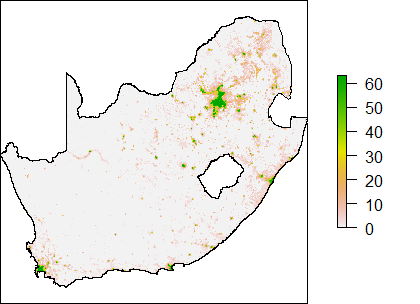
\includegraphics[width=1\linewidth]{figures/final} \caption{\label{final} Local Human Lights Image with Scale }\label{fig:final}
\end{figure}

\begin{figure}[H]
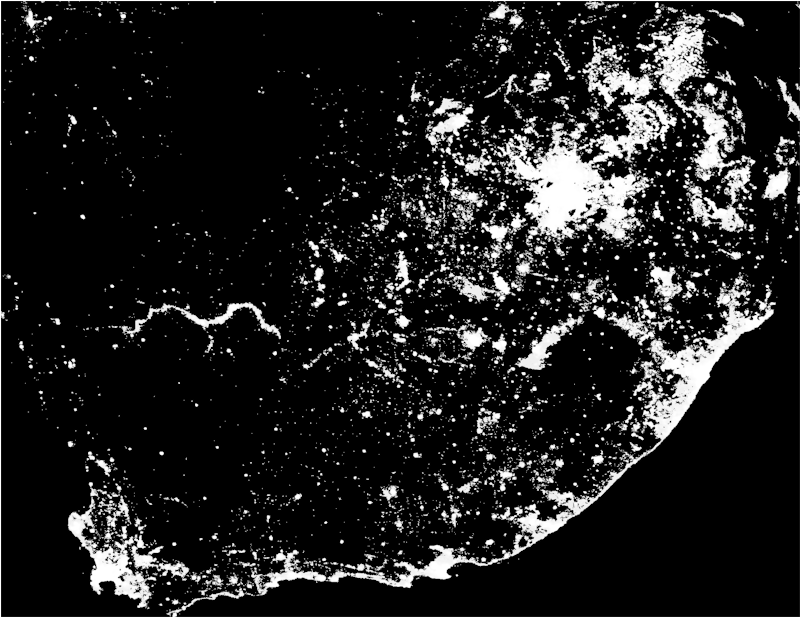
\includegraphics[width=1\linewidth]{figures/local_human_lights_image} \caption{\label{final_light} Local Human Lights Image}\label{fig:final_light}
\end{figure}

For an application such as the one described above, it is difficult to
convey and visualize results in an easy-to understand way. This is
compounded by the fact that common measures of prediction accuracy in a
random forest cannot be used for reasons mentioned earlier. Nonetheless,
we believe that our application does at least as well as Määttä \&
Lessmann (\protect\hyperlink{ref-maatta}{2019})'s. Those authors found
that the local human lights product increases the detection rate of
human settlements by 15.3\% in Africa over that of the stable lights
product.\footnote{Replicating these results fall outside of the scope of
  our paper, however.} Furthermore, and more importantly, the authors
found that the numbers of pixels lit in Africa increases from 2.95\%
using stable lights to 8.25\% using local human lights, an increase of
nearly 5 and a half percentage points. This increase is evident in our
analysis as well, if one visually compares Figures \ref{final} and
\ref{final_light}, which display the final local human lights images, to
Figure \ref{stable_no_noise} above.\footnote{As is evident, there
  remains potential in improving how to adequately display results for
  an application such as this. For instance, it would be good to be able
  to overlay the raster images with different colours so as to visualize
  the difference between the stable lights and local lights images on
  the same plot.} Overall, this would indicate that data at the lower
end of the luminosity spectrum, which would have been discarded or
replaced by an arbitrarily small value, can be used with confidence that
it is human-generated. Over and above this improvement, however, is that
the local human lights product also produces more data in general than
the stable lights product - a distinct advantage.

\hypertarget{discussion}{%
\section{\texorpdfstring{Discussion
\label{Discussion}}{Discussion }}\label{discussion}}

This paper extended the usage of a filtering methodology that separates
background noise from human-generated nightlight data to a specific
country - South Africa - for the years 2001 and 2011.Our results echo
those by Määttä \& Lessmann (\protect\hyperlink{ref-maatta}{2019}): the
RF algorithm introduces great improvements in classification accuracy
and thus greater accuracy in filtering out background noise from the
`Stable Lights' product. This allows the researcher to do away with the
need for quick-and-easy type fixes to filter out noisy data at the lower
end of the luminosity distribution. However, it is important to note
what this method does not achieve. For instance, the `Human Lights'
product does not address the issue of oversaturation at the higher end
of the luminosity spectrum. Likewise, its spatial resolution remains low
in comparison to more modern products such as the Visible Infrared
Imaging Radiometer Suite (VIIRS), and it is recommended to use these
products rather than the DMSP-OLS `Stable Lights' or `Human Lights'
products. Of course, this is not possible if one desires to study NL
data in the pre-VIIRS era. In those cases, the success in separating
noise from human-generated light at the lower end of the spectrum may
prove valuable in a variety of use-cases. For instance, if one were to
be interested in obtaining a rough measure of economic activity in
Sub-Saharan Africa, where data is often lacking and data is often
clustered in the lower end of the spectrum, then applying this filtering
technique might be extremely beneficial. Similarly, if one were to
attempt to create a Gini-type inequality index based on NL data, then
this strategy also holds promise. Lastly, it is reassuring that the
potential to further leverage remote sensing, big data and machine
learning to address the other challenges in these data sets remain as
well, and should be actively pursued so as to improve analysis accuracy
over and above what has been proposed in this paper.

{[}Words: 2952 excluding references, footnotes, bibliography and
abstract{]}

\newpage

\hypertarget{references}{%
\section*{References}\label{references}}
\addcontentsline{toc}{section}{References}

\hypertarget{refs}{}
\begin{CSLReferences}{1}{0}
\leavevmode\vadjust pre{\hypertarget{ref-chen2011}{}}%
Chen, X. \& Nordhaus, W.D. 2011. Using luminosity data as a proxy for
economic statistics. \emph{Proceedings of the National Academy of
Sciences}. 108(21):8589--8594.

\leavevmode\vadjust pre{\hypertarget{ref-elvidge1997}{}}%
Elvidge, C.D., Baugh, K.E., Kihn, E.A., Kroehl, H.W., Davis, E.R. \&
Davis, C.W. 1997a. Relation between satellite observed visible-near
infrared emissions, population, economic activity and electric power
consumption. \emph{International Journal of Remote Sensing}.
18(6):1373--1379.

\leavevmode\vadjust pre{\hypertarget{ref-elvidge1997relation}{}}%
Elvidge, C.D., Baugh, K.E., Kihn, E.A., Kroehl, H.W., Davis, E.R. \&
Davis, C.W. 1997b. Relation between satellite observed visible-near
infrared emissions, population, economic activity and electric power
consumption. \emph{International Journal of Remote Sensing}.
18(6):1373--1379.

\leavevmode\vadjust pre{\hypertarget{ref-elvidge2013viirs}{}}%
Elvidge, C.D., Baugh, K.E., Zhizhin, M. \& Hsu, F.-C. 2013. Why VIIRS
data are superior to DMSP for mapping nighttime lights.
\emph{Proceedings of the Asia-Pacific Advanced Network}. 35(0):62.

\leavevmode\vadjust pre{\hypertarget{ref-henderson2012}{}}%
Henderson, J.V., Storeygard, A. \& Weil, D.N. 2012. Measuring economic
growth from outer space. \emph{American economic review}.
102(2):994--1028.

\leavevmode\vadjust pre{\hypertarget{ref-ivan2020nlinequality}{}}%
Ivan, K., Holobâcă, I.-H., Benedek, J. \& Török, I. 2020. Potential of
night-time lights to measure regional inequality. \emph{Remote Sensing}.
12(1):33.

\leavevmode\vadjust pre{\hypertarget{ref-maatta}{}}%
Määttä, I. \& Lessmann, C. 2019. Human lights. \emph{Remote Sensing}.
11(19):2194.

\leavevmode\vadjust pre{\hypertarget{ref-mellander2015night}{}}%
Mellander, C., Lobo, J., Stolarick, K. \& Matheson, Z. 2015. Night-time
light data: A good proxy measure for economic activity? \emph{PloS one}.
10(10):e0139779.

\leavevmode\vadjust pre{\hypertarget{ref-mveyange2015}{}}%
Mveyange, A. 2015. \emph{Night lights and regional income inequality in
africa}. WIDER Working Paper.

\leavevmode\vadjust pre{\hypertarget{ref-pesaresi2016operating}{}}%
Pesaresi, M., Ehrlich, D., Ferri, S., Florczyk, A., Freire, S., Halkia,
M., Julea, A., Kemper, T., et al. 2016. Operating procedure for the
production of the global human settlement layer from landsat data of the
epochs 1975, 1990, 2000, and 2014. \emph{Publications Office of the
European Union}. 1--62.

\end{CSLReferences}

\newpage

\hypertarget{appendix}{%
\section*{Appendix}\label{appendix}}
\addcontentsline{toc}{section}{Appendix}

\begin{figure}[H]
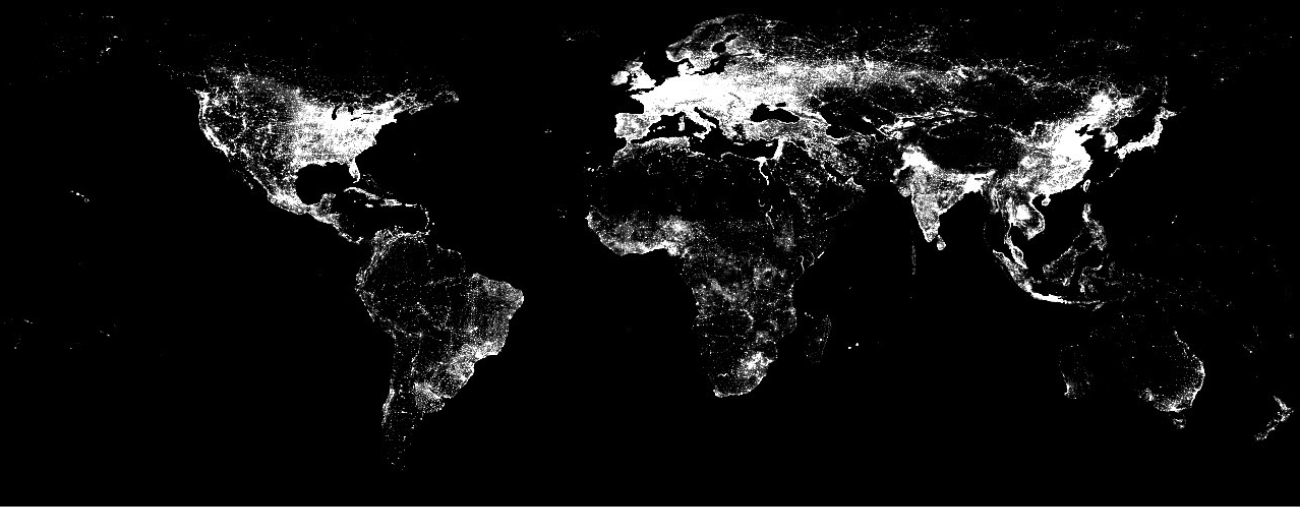
\includegraphics[width=1\linewidth]{figures/built_2011} \caption{\label{builtup} Interpolated 2014 built-up data from GHSL}\label{fig:builtup}
\end{figure}

\begin{figure}[H]
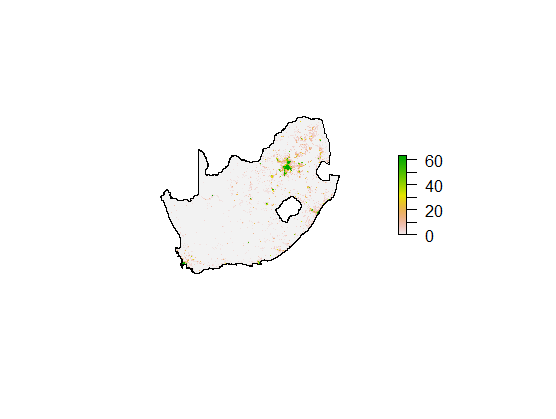
\includegraphics[width=1\linewidth]{figures/finalf14} \caption{\label{finalf142001} Final Local Human Lights Image for the F14 satellite for 2001}\label{fig:finalf142001}
\end{figure}

\begin{figure}[H]
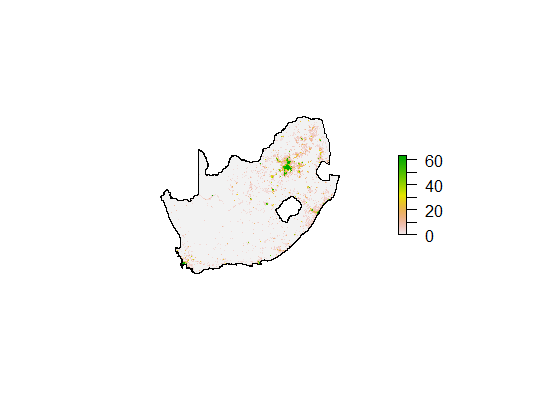
\includegraphics[width=1\linewidth]{figures/finalf15} \caption{\label{finalf152001} Final Local Human Lights Image for the F15 satellite for 2001}\label{fig:finalf152001}
\end{figure}

\bibliography{Tex/ref}





\end{document}
